\documentclass[11pt]{article}

\usepackage[T1]{fontenc}
\usepackage[utf8]{inputenc}
\usepackage{lmodern}
\usepackage[margin=0.8in]{geometry}
\usepackage{booktabs}
\usepackage{graphicx}
\usepackage{float}
\usepackage{hyperref}
\usepackage{array}
\usepackage{caption}
\usepackage{microtype}

\hypersetup{
  colorlinks=true,
  linkcolor=blue,
  citecolor=blue,
  urlcolor=blue,
  pdftitle={Experiment 1: CNN and Vision Transformer Skin-Lesion Benchmark}
}
\setlength{\parskip}{0.45em}
\setlength{\parindent}{0pt}
\renewcommand{\arraystretch}{1.15}

\title{\textbf{Experiment 1: CNN--Vision Transformer Comparison}\\
\large Skin-Lesion Classification Performance, Transfer, and Computational Cost}
\author{Research report}
\date{12 November 2026}

\begin{document}
\maketitle

\begin{abstract}
This report compares pretrained ResNet-50 and ViT-Base/16 classifiers for seven-class skin-lesion image classification. Each architecture was evaluated with a frozen pretrained backbone and with full fine-tuning. All four configurations used the same lesion-grouped HAM10000 train, validation, and held-out test partitions. On the 1,431-image HAM10000 test partition, fine-tuned ViT-B/16 achieved the highest macro-F1 (0.705), accuracy (0.838), and one-vs-rest macro ROC-AUC (0.960); its melanoma sensitivity was 0.667 (106/159). On the 1,141 mapped PAD-UFES-20 images, all models performed substantially worse and melanoma sensitivity ranged from 0.038 to 0.212. The latter result is consistent with a difficult transfer setting but does not isolate imaging-domain shift from other dataset differences. ResNet-50 inference was about twice as fast and its checkpoint about 3.6 times smaller than ViT-B/16. These are single-seed results, and the external melanoma estimate is based on only 52 images. They support a limited empirical comparison, not a clinical-use claim.
\end{abstract}

\section{Research question and scope}

The question for this experiment is: under which training conditions do a convolutional neural network and a Vision Transformer offer a useful balance of classification performance and computational cost on skin-lesion images? The comparison follows the Experiment 1 scope in the project plan. It evaluates two existing architectures and does not claim a new architecture or a universally superior model.

The completed configurations are pretrained ResNet-50 and ViT-B/16, each used as (1) a frozen feature extractor with a newly trained classification head and (2) a fully fine-tuned model. Training from scratch was not run. The separate feature-fusion experiment in the planning document is outside the scope of this report.

\section{Data and partitions}

\subsection{HAM10000}

HAM10000 contains 10,015 indexed and readable dermoscopic images in seven diagnostic classes \cite{tschandl2018}. The data are imbalanced: the source metadata contains 6,705 nevus (nv) images, compared with 115 dermatofibroma (df) images. Partitions were fixed before training using nested stratified group folds with \texttt{lesion\_id} as the grouping key and seed 42. The resulting partitions were:

\begin{center}
\begin{tabular}{lrr}
\toprule
Partition & Images & Lesion groups\\
\midrule
Train & 7,153 & 5,336\\
Validation & 1,431 & 1,067\\
Held-out test & 1,431 & 1,067\\
\bottomrule
\end{tabular}
\end{center}

No lesion group appears in more than one partition. The metadata does not provide reliable patient identifiers for every HAM10000 image, so lesion-level grouping does not establish patient-level independence. The held-out test partition was not used for training or checkpoint selection.

\subsection{PAD-UFES-20 external evaluation}

PAD-UFES-20 contains clinical photographs collected using smartphones, whereas HAM10000 consists of dermoscopic images \cite{pacheco2020}. The configured label harmonization retained BCC $\rightarrow$ bcc, MEL $\rightarrow$ mel, and NEV $\rightarrow$ nv. Of 2,298 indexed images, 1,141 readable examples had one of these labels: 845 bcc, 52 mel, and 244 nv. The other 1,157 records were excluded (ACK: 730, SCC: 192, SEK: 235). The mapped subset includes 720 patient groups.

All four selected checkpoints were evaluated on this mapped external subset after training and internal evaluation. No model or hyperparameter was selected using these external results. An exact SHA-256 comparison found no byte-identical images between the indexed HAM10000 and PAD-UFES-20 image sets; perceptual or near-duplicate overlap was not checked.

\section{Models and training procedure}

The CNN was torchvision ResNet-50~\cite{he2016} with ImageNet-1K V2 weights (23,522,375 parameters). The transformer was torchvision ViT-Base/16~\cite{dosovitskiy2021} with ImageNet-1K V1 weights (85,804,039 parameters). The frozen configurations trained 14,343 ResNet parameters and 5,383 ViT parameters; both fine-tuning configurations updated all model parameters.

All runs used 224 by 224 inputs, batch size 4, automatic mixed precision (FP16), ImageNet channel normalization, and the same random horizontal and vertical flips and rotations up to 15 degrees. Training used AdamW, class-weighted cross-entropy (weights calculated from the training partition), weight decay $10^{-4}$, and validation macro-F1 for checkpoint selection. The maximum was 20 epochs with early-stopping patience 4. Frozen-head learning rate was $10^{-3}$; fine-tuning used $10^{-5}$ for the backbone and $10^{-4}$ for the head. A reduce-on-plateau schedule used factor 0.2 and patience 2. Each configuration used seed 42.

Runs executed on an NVIDIA GeForce RTX 4050 Laptop GPU. The recorded environment was PyTorch 2.11.0+cu128, torchvision 0.26.0+cu128, and CUDA 12.8. The training summaries show that the best validation macro-F1 checkpoints occurred at epoch 19 for frozen ResNet-50 (0.552), epoch 9 for frozen ViT-B/16 (0.637), epoch 8 for fine-tuned ResNet-50 (0.694), and epoch 8 for fine-tuned ViT-B/16 (0.779).

\section{Evaluation}

Primary predictive metrics are macro-F1, balanced accuracy (mean recall across classes with true support), and per-class recall. Accuracy, one-vs-rest macro specificity, and one-vs-rest macro ROC-AUC are also reported. AUC uses the predicted softmax score for each supported class. External macro metrics average over the three mapped classes with true support. The classifier still has seven HAM10000 output classes; an external prediction in one of the four unmapped classes counts as an error.

The paired bootstrap resampled the same evaluation images for the CNN and ViT, stratified by true class, for 2,000 repetitions. Reported percentile 95\% intervals quantify case-sampling uncertainty for these fixed checkpoints; they do not quantify training-seed variation. The resampling unit was the image rather than the lesion or patient, so correlations among images from a shared lesion or patient are not modeled.

Inference timing used five warm-up batches and synchronized GPU measurements at batch size 4. Per-image latency includes host-to-device transfer and the model forward pass, but excludes image decoding. Training time is the recorded sum of training epochs; validation is reported separately in the run summaries. Memory is the recorded peak allocated GPU memory during training and peak process resident set size (RSS). Checkpoint sizes are the saved \texttt{best.pt} file sizes.

\section{Results}

\subsection{HAM10000 held-out test performance}

Table~\ref{tab:internal} reports all four configurations on the same 1,431-image test partition. Fine-tuned ViT-B/16 had the highest macro-F1, accuracy, and macro ROC-AUC. Its balanced accuracy (0.665) was close to fine-tuned ResNet-50 (0.662).

\begin{table}[H]
\centering
\small
\caption{HAM10000 held-out test results. Values are proportions except melanoma sensitivity, which is shown as a percentage.}
\label{tab:internal}
\begin{tabular}{llrrrrrr}
\toprule
Model & Strategy & Accuracy & Macro-F1 & Bal. acc. & Macro spec. & Macro AUC & Mel. sens.\\
\midrule
ResNet-50 & Frozen & 0.748 & 0.549 & 0.537 & 0.946 & 0.904 & 49.1\%\\
ViT-B/16 & Frozen & 0.794 & 0.605 & 0.604 & 0.951 & 0.945 & 50.3\%\\
ResNet-50 & Fine-tuned & 0.806 & 0.648 & 0.662 & 0.955 & 0.935 & 56.6\%\\
ViT-B/16 & Fine-tuned & \textbf{0.838} & \textbf{0.705} & \textbf{0.665} & \textbf{0.959} & \textbf{0.960} & \textbf{66.7\%}\\
\bottomrule
\end{tabular}
\end{table}

The full class-wise recalls are shown in Table~\ref{tab:internal-recall}. Fine-tuned ViT-B/16 detected 106 of 159 melanoma images (53 false negatives). Fine-tuned ResNet-50 detected 90 of 159 (69 false negatives). The rare-class supports are small: 17 df and 20 vasc images in the test partition.

\begin{table}[H]
\centering
\small
\caption{HAM10000 test recall/sensitivity by class (percent).}
\label{tab:internal-recall}
\begin{tabular}{lrrrrr}
\toprule
Class & Support & ResNet frozen & ViT frozen & ResNet fine-tuned & ViT fine-tuned\\
\midrule
akiec & 46 & 50.0 & 50.0 & 52.2 & 47.8\\
bcc   & 74 & 44.6 & 73.0 & 74.3 & 70.3\\
bkl   & 157 & 56.1 & 58.6 & 64.3 & 65.6\\
df    & 17 & 29.4 & 35.3 & 41.2 & 47.1\\
mel   & 159 & 49.1 & 50.3 & 56.6 & 66.7\\
nv    & 958 & 86.7 & 90.6 & 89.8 & 93.2\\
vasc  & 20 & 60.0 & 65.0 & 85.0 & 75.0\\
\bottomrule
\end{tabular}
\end{table}

\subsection{PAD-UFES-20 external performance}

The external results were substantially lower than the internal test results (Table~\ref{tab:external}). Frozen ViT-B/16 had the highest external accuracy and macro-F1, while fine-tuned ViT-B/16 had the highest balanced accuracy and macro AUC. None of the configurations had melanoma sensitivity above 0.212 on the 52 mapped melanoma images.

\begin{table}[H]
\centering
\small
\caption{PAD-UFES-20 mapped external subset ($n=1,141$). Metrics are calculated over bcc, mel, and nv.}
\label{tab:external}
\begin{tabular}{llrrrrr}
\toprule
Model & Strategy & Accuracy & Macro-F1 & Bal. acc. & Macro spec. & Macro AUC\\
\midrule
ResNet-50 & Frozen & 0.422 & 0.407 & 0.441 & 0.875 & 0.766\\
ViT-B/16 & Frozen & \textbf{0.502} & \textbf{0.444} & 0.381 & \textbf{0.924} & 0.806\\
ResNet-50 & Fine-tuned & 0.340 & 0.327 & 0.352 & 0.876 & 0.733\\
ViT-B/16 & Fine-tuned & 0.480 & 0.433 & \textbf{0.470} & 0.886 & \textbf{0.817}\\
\bottomrule
\end{tabular}
\end{table}

\begin{table}[H]
\centering
\small
\caption{PAD-UFES-20 external recall/sensitivity by mapped class (percent).}
\label{tab:external-recall}
\begin{tabular}{lrrrrr}
\toprule
Class & Support & ResNet frozen & ViT frozen & ResNet fine-tuned & ViT fine-tuned\\
\midrule
bcc & 845 & 33.3 & 50.2 & 24.7 & 38.8\\
mel & 52  & 21.2 & 3.8  & 9.6  & 15.4\\
nv  & 244 & 77.9 & 60.2 & 71.3 & 86.9\\
\bottomrule
\end{tabular}
\end{table}

\subsection{Paired CNN--ViT comparisons}

Table~\ref{tab:paired} reports ViT minus ResNet differences within each training strategy. On the internal test set, the macro-F1 intervals favored ViT for both strategies. For fine-tuning, the balanced-accuracy difference was small and its interval included zero. On PAD-UFES-20, fine-tuned ViT had higher macro-F1 and balanced accuracy in this paired analysis. Among frozen models, the external macro-F1 interval includes zero, while the balanced-accuracy difference favors ResNet. These comparisons concern the fixed seed-42 checkpoints and the sampled images, not variation across retraining.

\begin{table}[H]
\centering
\small
\caption{Paired, true-class-stratified bootstrap differences (ViT minus ResNet), in percentage points; 2,000 repetitions.}
\label{tab:paired}
\begin{tabular}{llrrrr}
\toprule
Split & Strategy & $\Delta$ Macro-F1 & 95\% interval & $\Delta$ Bal. acc. & 95\% interval\\
\midrule
HAM test & Frozen & +5.64 & [+0.38, +10.70] & +6.70 & [+1.26, +11.87]\\
HAM test & Fine-tuned & +5.66 & [+1.28, +9.93] & +0.32 & [-4.24, +4.45]\\
PAD external & Frozen & +3.75 & [-0.39, +7.94] & -6.00 & [-10.87, -1.35]\\
PAD external & Fine-tuned & +10.54 & [+7.02, +14.07] & +11.81 & [+7.83, +15.83]\\
\bottomrule
\end{tabular}
\end{table}

\subsection{Training and inference cost}

ResNet-50 inference was about twice as fast as ViT-B/16 on the held-out test benchmark, with materially smaller checkpoints. Fine-tuning ViT-B/16 took the longest. The measurements are from this laptop GPU, one seed, batch size 4, and 224-pixel inputs, so they should be interpreted as observed run costs rather than hardware-independent model properties.

\begin{table}[H]
\centering
\scriptsize
\caption{Observed resource use. Test latency and throughput are measured on the HAM10000 test benchmark.}
\label{tab:compute}
\resizebox{\textwidth}{!}{%
\begin{tabular}{llrrrrrrrr}
\toprule
Model & Strategy & Trainable params. & Train min. & Validation (s) & Train GPU peak (MB) & Train RSS peak (MB) & Test ms/image & Test images/s & Checkpoint (MB)\\
\midrule
ResNet-50 & Frozen & 14,343 & 19.7 & 240.4 & 1,198 & 1,769 & 3.91 & 255.8 & 94.4\\
ViT-B/16 & Frozen & 5,383 & 16.3 & 207.0 & 371 & 1,896 & 7.95 & 125.8 & 343.3\\
ResNet-50 & Fine-tuned & 23,522,375 & 22.2 & 160.0 & 1,473 & 2,002 & 4.01 & 249.3 & 94.4\\
ViT-B/16 & Fine-tuned & 85,804,039 & 32.7 & 153.9 & 1,661 & 1,932 & 8.15 & 122.7 & 343.3\\
\bottomrule
\end{tabular}}
\end{table}

Peak allocated GPU memory during inference was 123 MB for ResNet-50 and 361 MB for ViT-B/16. Training time and validation time are reported separately. The ResNet checkpoint is approximately 94.4 MB; the ViT checkpoint is approximately 343.3 MB.

\section{Discussion}

On the internal HAM10000 test partition, fine-tuned ViT-B/16 provided the strongest macro-F1, accuracy, and AUC, and its melanoma sensitivity exceeded that of the other tested configurations. Its balanced accuracy was nearly tied with fine-tuned ResNet-50, however, and the paired interval for their balanced-accuracy difference included zero. ResNet-50 offered faster inference and substantially smaller checkpoint storage. The choice therefore depends on whether the higher observed macro-F1 and melanoma recall justify the added inference and storage costs for the intended research setting.

The external results show that internal test performance did not transfer directly to the mapped PAD-UFES-20 images. The two datasets differ in image acquisition, and the external set contains only three harmonized classes with a particularly small melanoma sample. These results therefore indicate performance under a combined dataset, label, and imaging-domain shift; they do not identify which source caused the drop. The poor external melanoma sensitivity is a central finding and rules out interpreting the internal melanoma results as evidence of reliable external detection.

The external results also show why overall accuracy alone is insufficient. Frozen ViT-B/16 had the highest external accuracy and macro-F1, but its melanoma sensitivity was only 3.8\%. Fine-tuned ViT-B/16 had the strongest external balanced accuracy of the four, yet detected only 8 of 52 melanoma images. The high macro-specificity values do not offset these class-wise misses.

\section{Limitations}

\begin{itemize}
  \item Each architecture--strategy configuration was trained once, with seed 42. Bootstrap intervals quantify resampling of evaluation images for these checkpoints, not between-seed training variability.
  \item HAM10000 partitions were grouped by lesion, not patient. The image-level bootstrap also does not account for dependence among images from the same lesion.
  \item The external set has 52 mapped melanoma images from 720 patient groups overall. Bootstrap resampling was image-based, not patient-clustered, and may understate uncertainty when multiple images belong to one patient.
  \item Only BCC, MEL, and NEV were mapped from PAD-UFES-20. This subset is not a complete PAD-UFES-20 benchmark; predictions to the four unmapped HAM classes count as errors.
  \item Exact byte-level overlap was checked, but visually similar or re-encoded duplicates were not.
  \item Training from scratch, additional seeds, and external patient-clustered uncertainty estimates were not part of the completed runs.
  \item Results from public image datasets do not establish clinical safety, utility, or deployment readiness. These classifiers are not diagnostic replacements for clinicians.
\end{itemize}

\section{Conclusion}

For the tested seed-42 runs, fine-tuned ViT-B/16 was strongest on HAM10000 macro-F1 and melanoma sensitivity, while ResNet-50 had roughly twice the inference throughput and a smaller checkpoint. External PAD-UFES-20 performance was much weaker, especially for melanoma, and reversed some class and strategy rankings. The evidence supports a bounded conclusion: model-family trade-offs depend on training strategy and evaluation domain. Repeated seeds and patient- or lesion-clustered uncertainty estimates are needed before making stronger comparative claims.

\section*{Reproducibility artifacts}

Aggregate metrics and paired bootstrap tables are saved at \path{results/tables/test_aggregate.csv}, \path{results/tables/test_paired_bootstrap.csv}, \path{results/tables/external_aggregate.csv}, and \path{results/tables/external_paired_bootstrap.csv}. Per-run prediction files, class metrics, confusion matrices, and JSON summaries are under \path{results/evaluations/}. Training summaries, histories, copied configurations, and checkpoints are under \path{results/runs/}. The fixed data partitions are under \path{data/splits/}.

\appendix
\section{Confusion matrices}

The following figures are the saved per-run confusion matrices. The external figures retain the seven classifier output labels; only bcc, mel, and nv occur as true classes in the mapped external subset.

\begin{figure}[p]
\centering
\begin{minipage}{0.48\textwidth}\centering
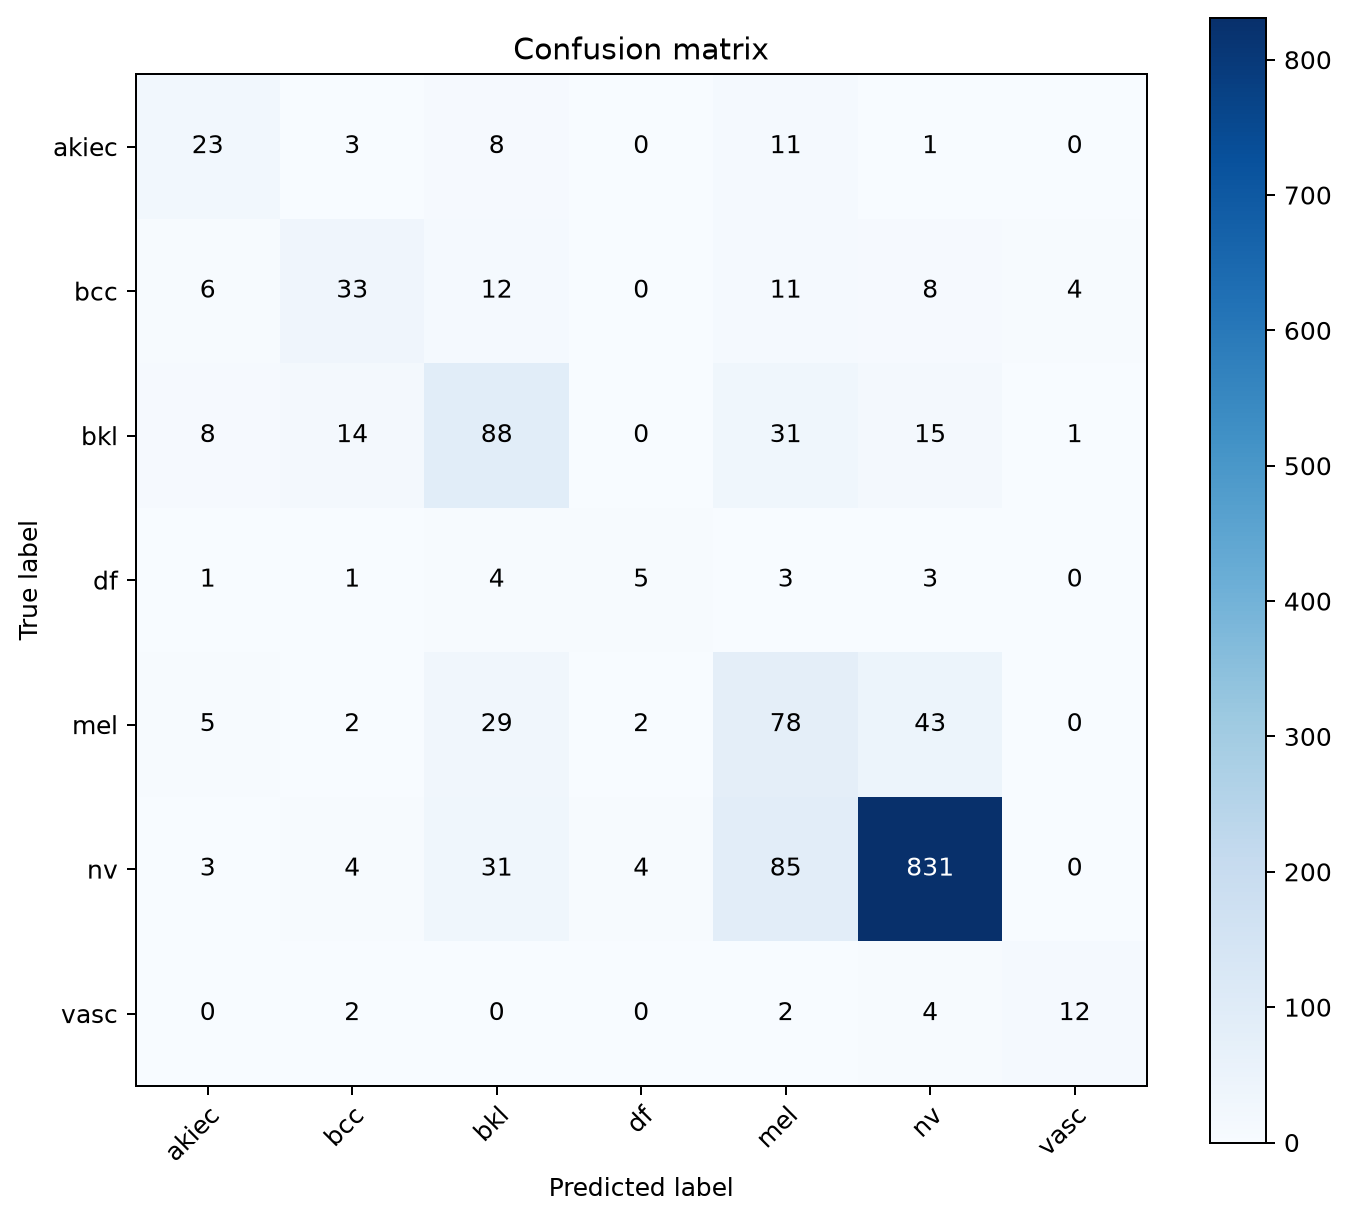
\includegraphics[width=\linewidth]{results/evaluations/resnet50_frozen_seed42_20261112T153434Z/test/test_confusion_matrix.png}
\caption*{(a) ResNet-50, frozen}
\end{minipage}\hfill
\begin{minipage}{0.48\textwidth}\centering
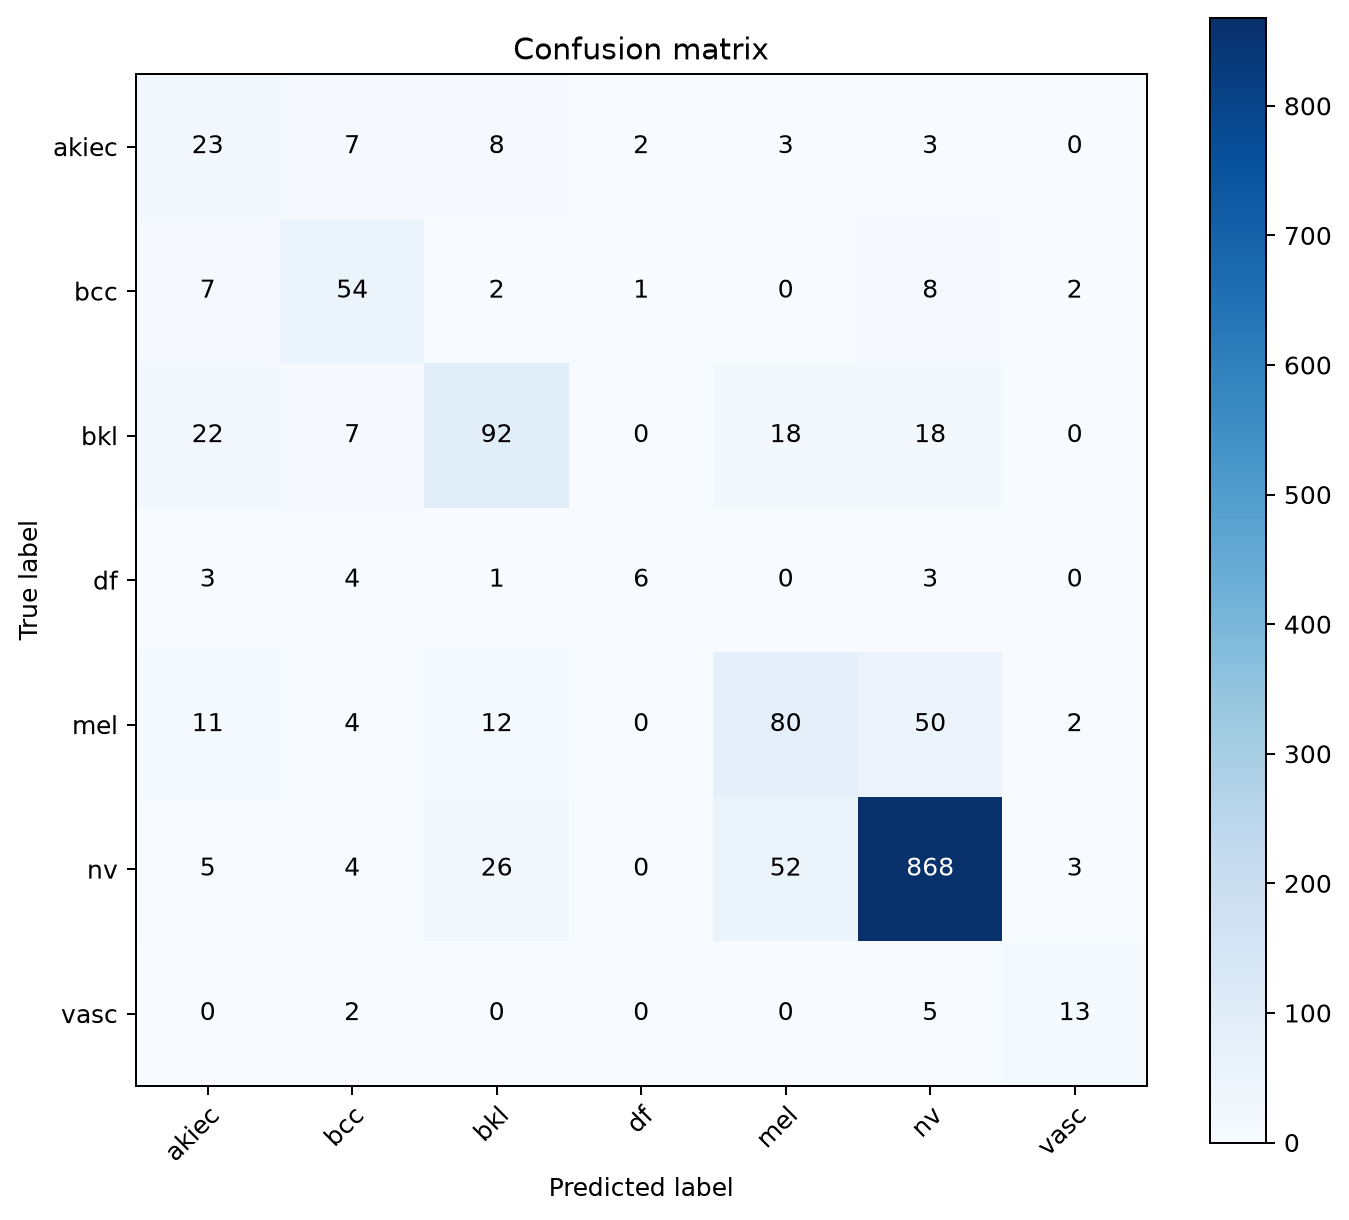
\includegraphics[width=\linewidth]{results/evaluations/vit_b_16_frozen_seed42_20261112T160102Z/test/test_confusion_matrix.png}
\caption*{(b) ViT-B/16, frozen}
\end{minipage}

\vspace{0.5cm}

\begin{minipage}{0.48\textwidth}\centering
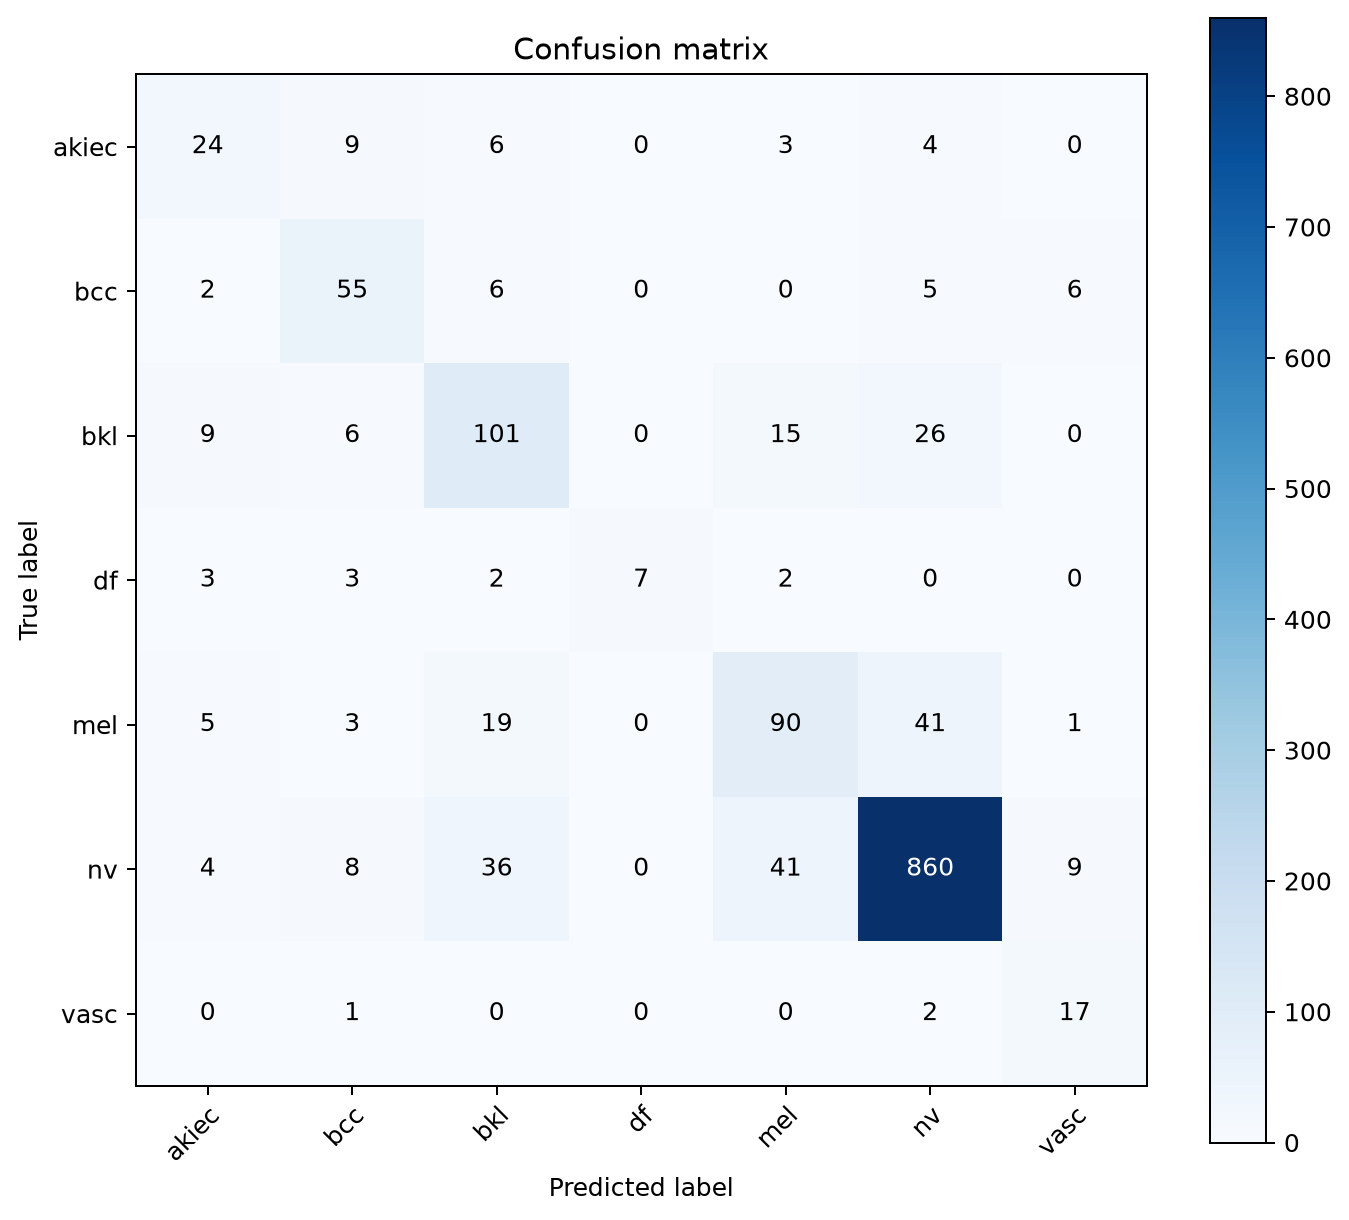
\includegraphics[width=\linewidth]{results/evaluations/resnet50_finetune_seed42_20261112T162123Z/test/test_confusion_matrix.png}
\caption*{(c) ResNet-50, fine-tuned}
\end{minipage}\hfill
\begin{minipage}{0.48\textwidth}\centering
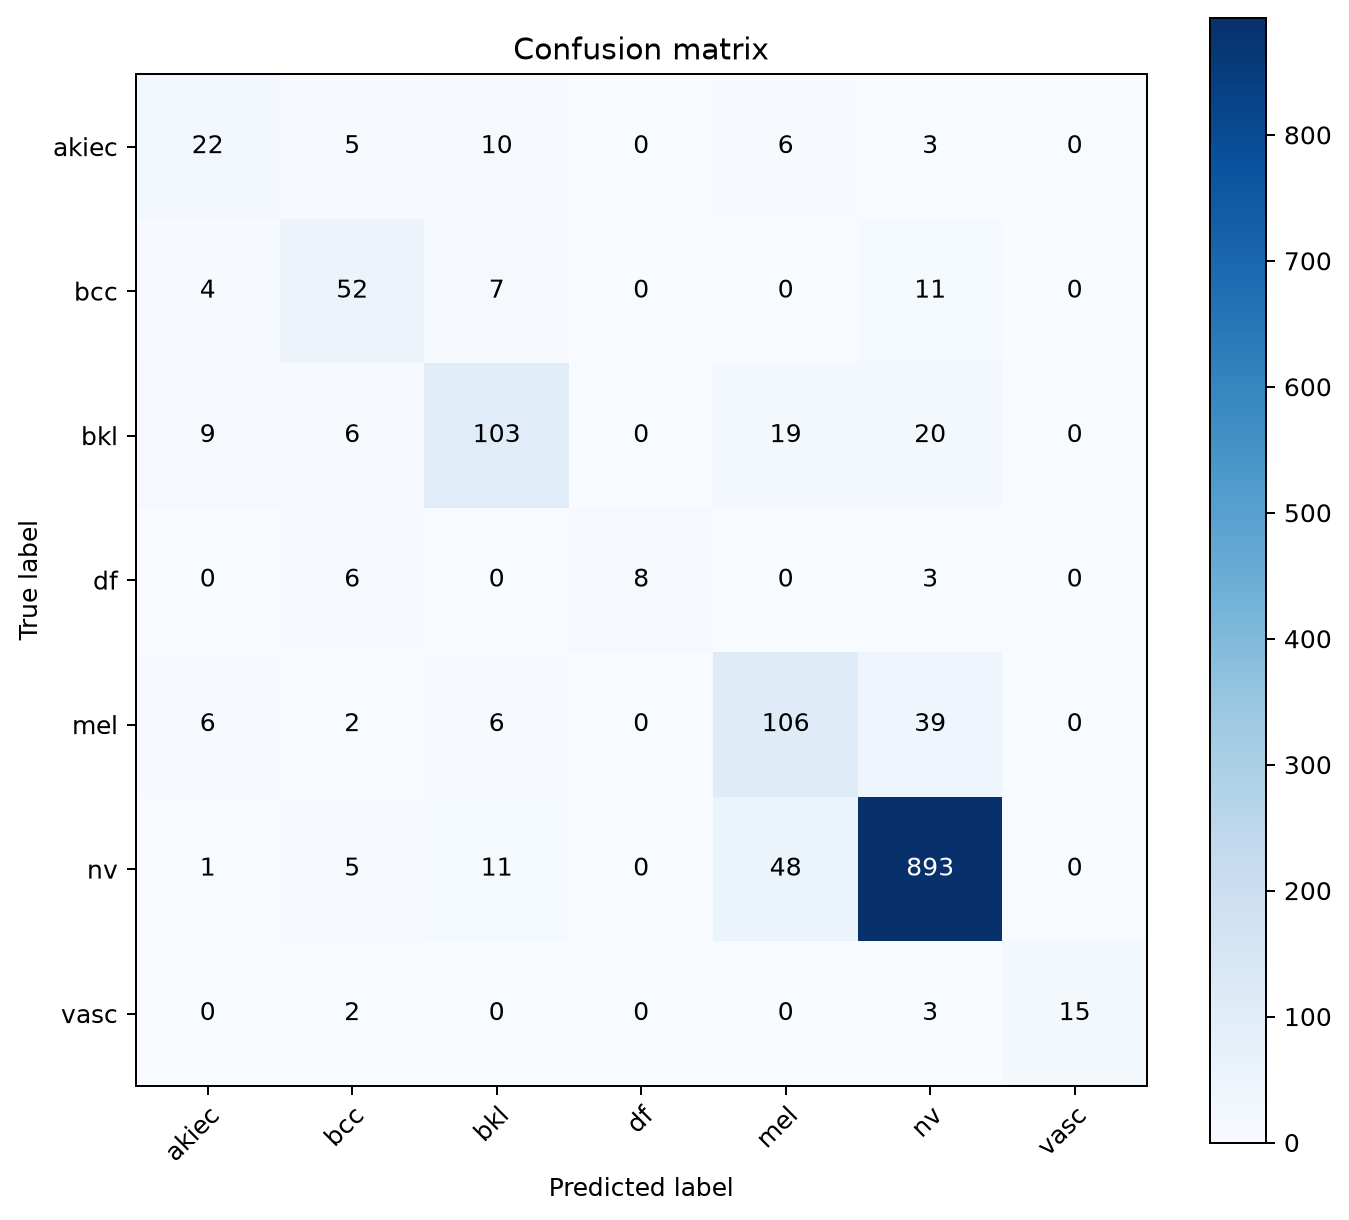
\includegraphics[width=\linewidth]{results/evaluations/vit_b_16_finetune_seed42_20261112T164641Z/test/test_confusion_matrix.png}
\caption*{(d) ViT-B/16, fine-tuned}
\end{minipage}
\caption{HAM10000 held-out test confusion matrices.}
\end{figure}

\begin{figure}[p]
\centering
\begin{minipage}{0.48\textwidth}\centering
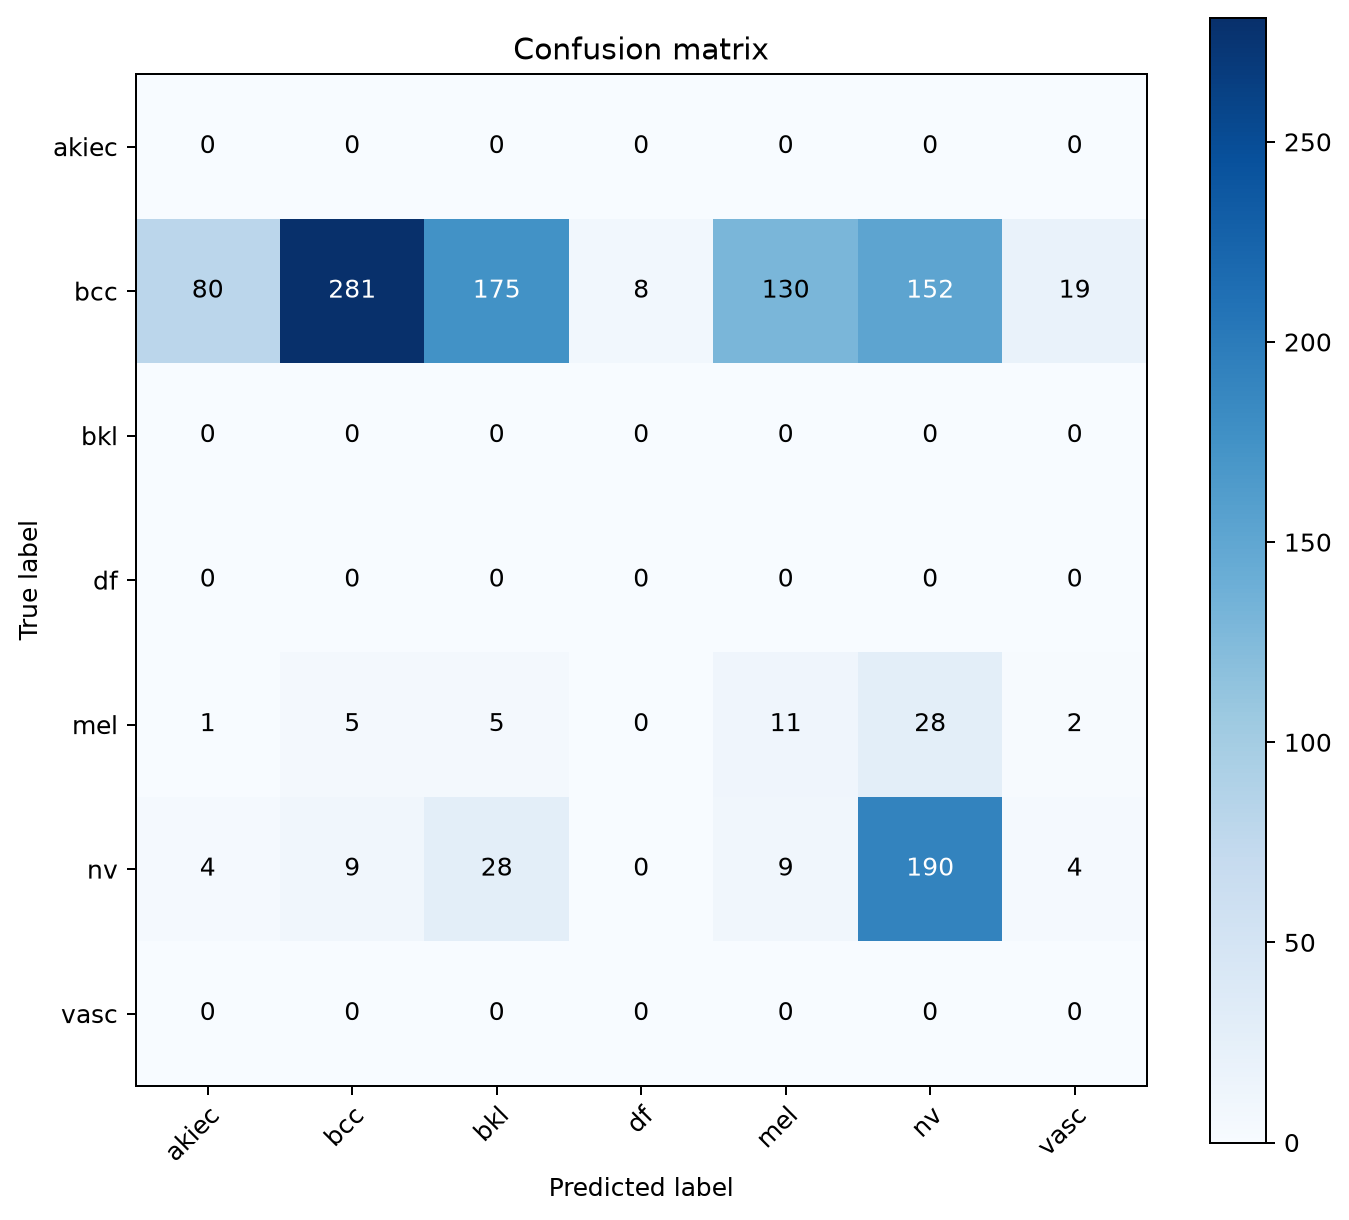
\includegraphics[width=\linewidth]{results/evaluations/resnet50_frozen_seed42_20261112T153434Z/external/external_confusion_matrix.png}
\caption*{(a) ResNet-50, frozen}
\end{minipage}\hfill
\begin{minipage}{0.48\textwidth}\centering
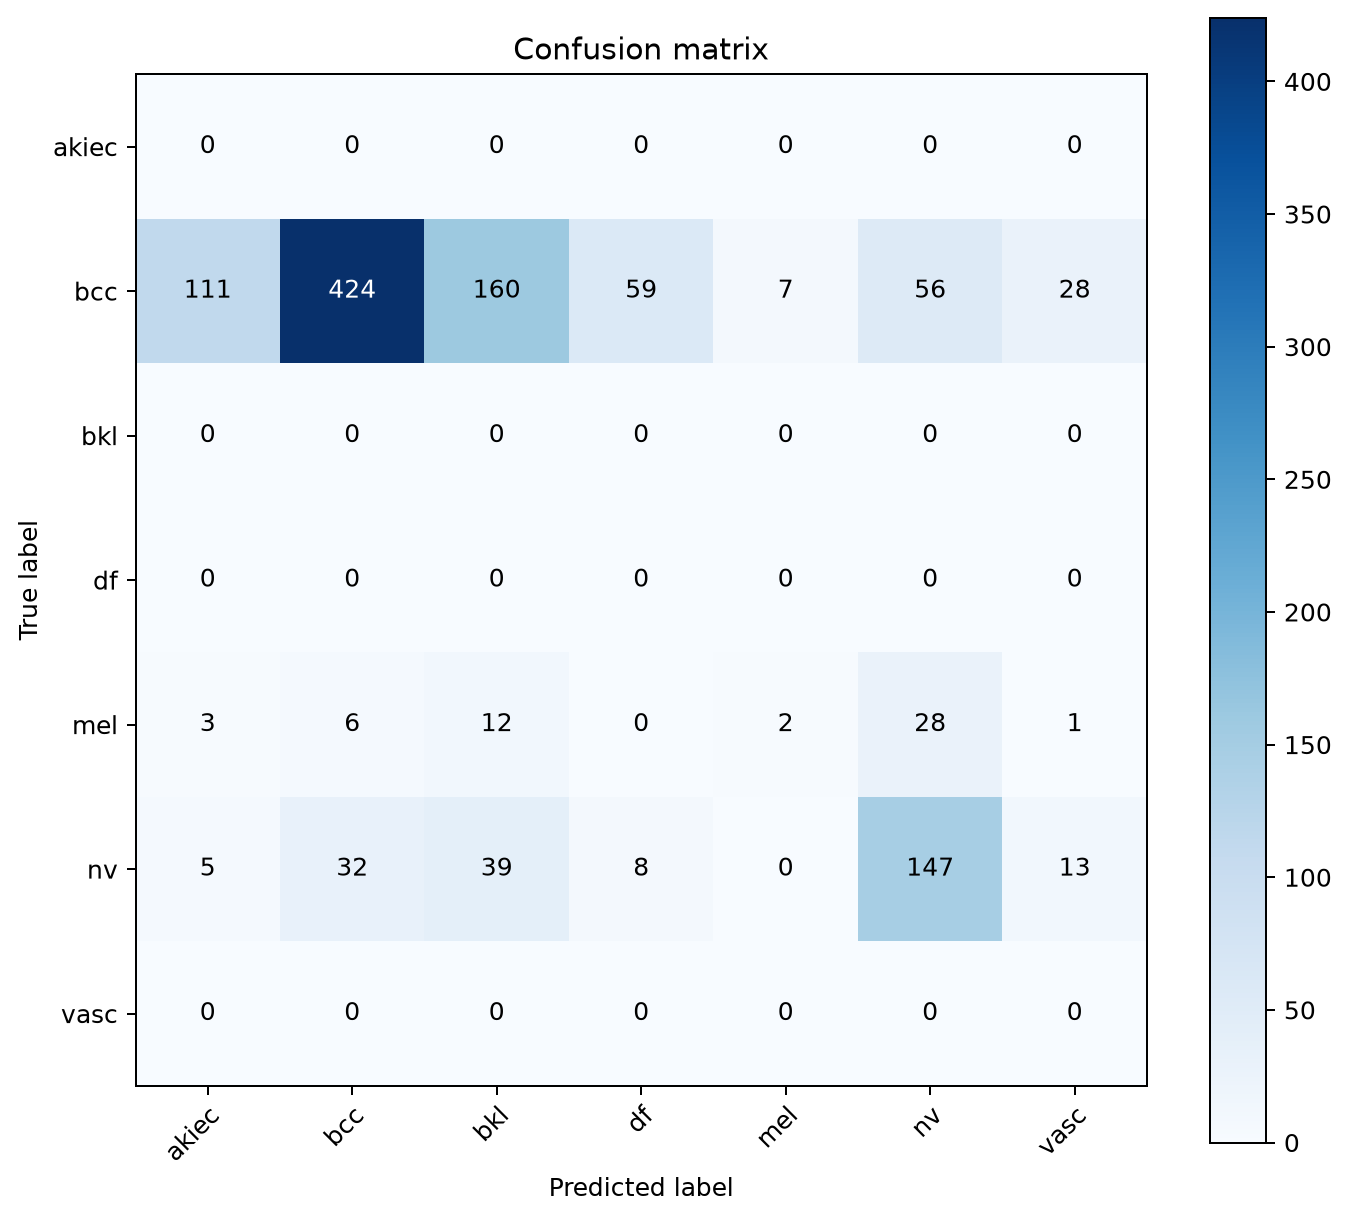
\includegraphics[width=\linewidth]{results/evaluations/vit_b_16_frozen_seed42_20261112T160102Z/external/external_confusion_matrix.png}
\caption*{(b) ViT-B/16, frozen}
\end{minipage}

\vspace{0.5cm}

\begin{minipage}{0.48\textwidth}\centering
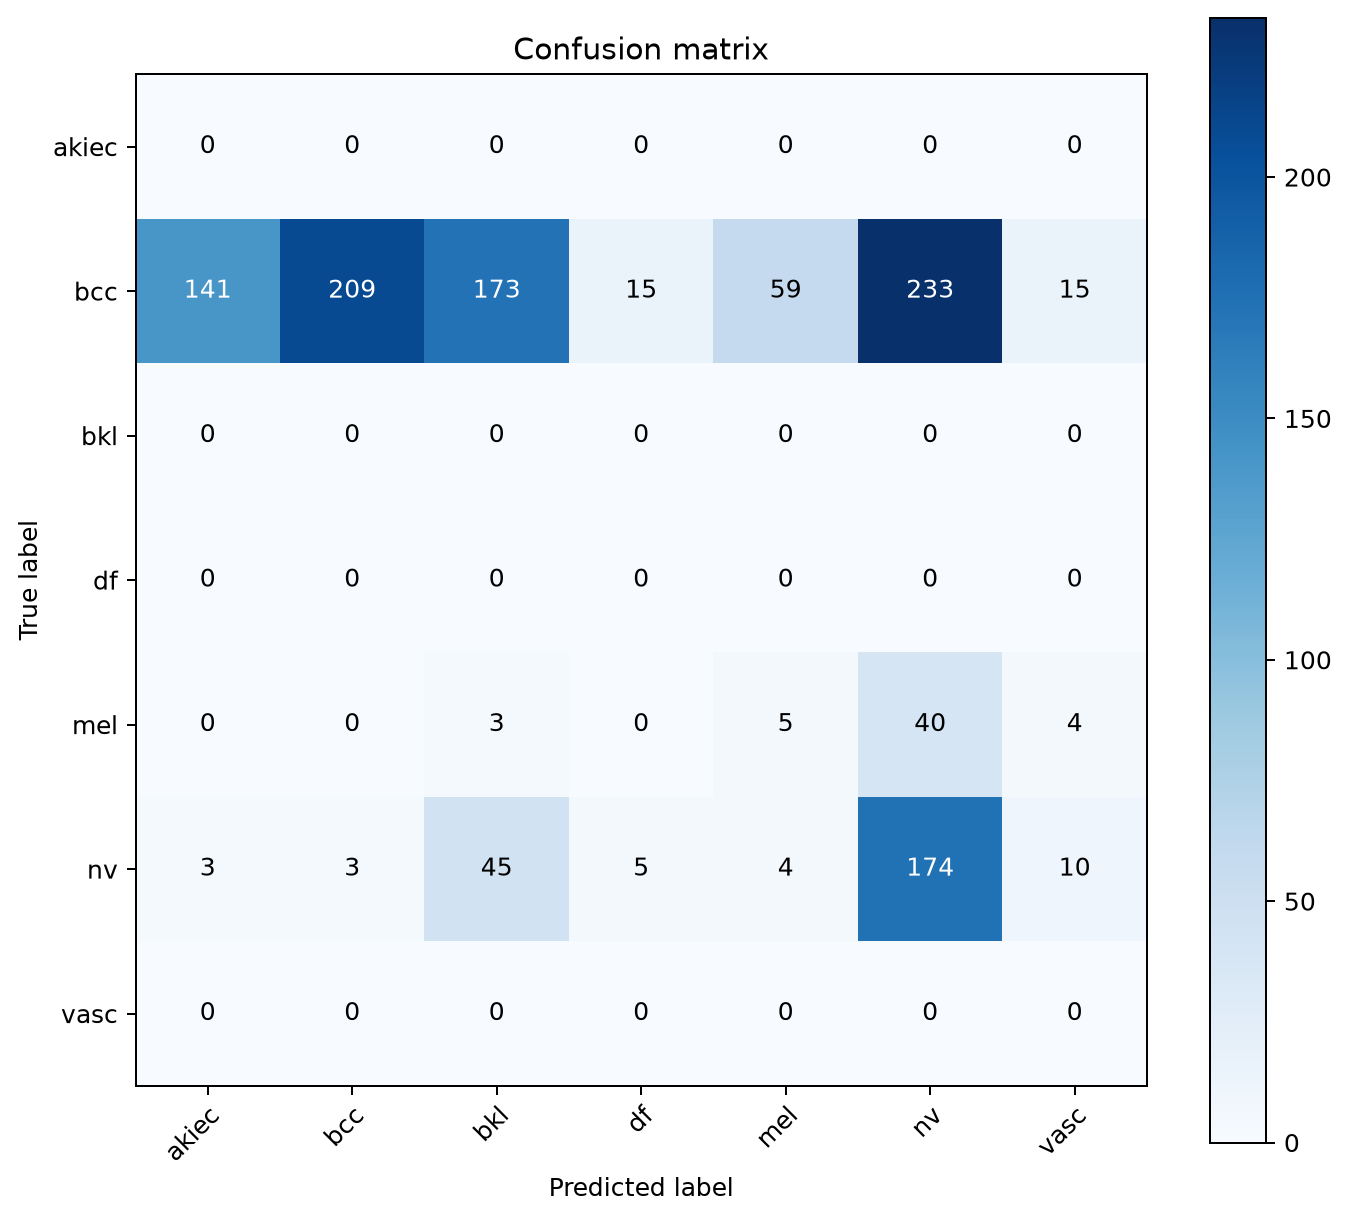
\includegraphics[width=\linewidth]{results/evaluations/resnet50_finetune_seed42_20261112T162123Z/external/external_confusion_matrix.png}
\caption*{(c) ResNet-50, fine-tuned}
\end{minipage}\hfill
\begin{minipage}{0.48\textwidth}\centering
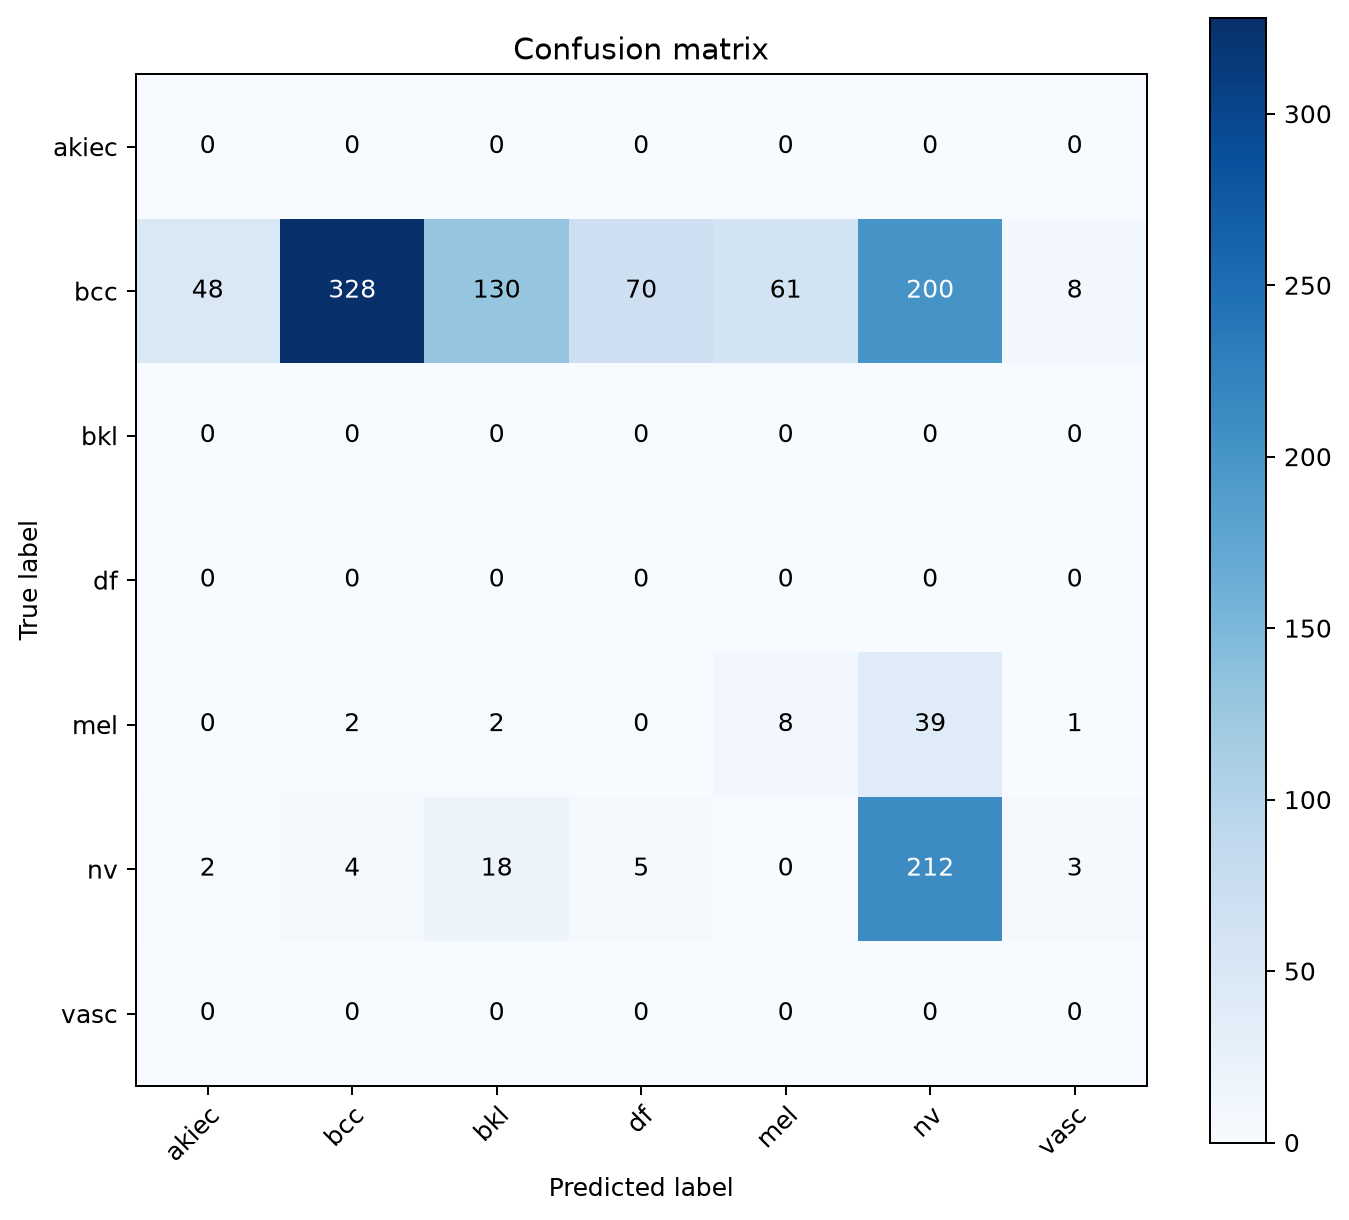
\includegraphics[width=\linewidth]{results/evaluations/vit_b_16_finetune_seed42_20261112T164641Z/external/external_confusion_matrix.png}
\caption*{(d) ViT-B/16, fine-tuned}
\end{minipage}
\caption{PAD-UFES-20 mapped-subset confusion matrices.}
\end{figure}

\begin{thebibliography}{9}
\bibitem{tschandl2018}
P. Tschandl, C. Rosendahl, and H. Kittler.
\newblock The HAM10000 dataset, a large collection of multi-source dermatoscopic images of common pigmented skin lesions.
\newblock \emph{Scientific Data}, 5:180161, 2018.
\newblock \url{https://doi.org/10.1038/sdata.2018.161}.

\bibitem{pacheco2020}
A. G. C. Pacheco et al.
\newblock PAD-UFES-20: A skin lesion dataset composed of patient data and clinical images collected from smartphones.
\newblock \emph{Data in Brief}, 32:106221, 2020.
\newblock \url{https://doi.org/10.1016/j.dib.2020.106221}.

\bibitem{he2016}
K. He, X. Zhang, S. Ren, and J. Sun.
\newblock Deep residual learning for image recognition.
\newblock In \emph{Proceedings of the IEEE Conference on Computer Vision and Pattern Recognition}, pages 770--778, 2016.
\newblock \url{https://openaccess.thecvf.com/content_cvpr_2016/html/He_Deep_Residual_Learning_CVPR_2016_paper.html}.

\bibitem{dosovitskiy2021}
A. Dosovitskiy et al.
\newblock An image is worth 16x16 words: Transformers for image recognition at scale.
\newblock In \emph{International Conference on Learning Representations}, 2021.
\newblock \url{https://openreview.net/forum?id=YicbFdNTTy}.
\end{thebibliography}

\end{document}
